\documentclass[11pt,a4paper]{report}
\usepackage[utf8]{inputenc}
\usepackage[french]{babel}
\usepackage[T1]{fontenc}
\usepackage{amsmath}
\usepackage{amsfonts}
\usepackage{amssymb}
\usepackage{graphicx}
\usepackage{minted}
\usepackage{parskip}
\usepackage{fullpage}
\usepackage{amsthm}
\usepackage{mathtools}
\usepackage{tikz}
\usetikzlibrary{trees}

\author{Sylvain Julmy}
\title{ProgAlg - Résumé}

\newcommand{\Uu}[1]{\overset{\nearrow}{#1}}
\newcommand{\Dd}[1]{\overset{\searrow}{#1}}

\begin{document}

\maketitle

\chapter{Introduction} % (fold)
\label{cha:Introduction}

\paragraph*{Concurrent computing :} A form of computing in which programs are designed as a collections of interaction computational processes that may be executed in parallel.

\paragraph*{Parallel computing :} A form of computing in which many calculations are carried out simultaneously, operating on the principle that large problems can be divided into smaller ones. The most popular form is the multi-core processors.

\paragraph*{Distributed computing :} Any computing that involves multiple computers remote from each other that each have a role in a computation problem or information processing. Motivation : High performance (HPC) to avoid processing issue (compute faster) and memory issue (compute larger problems).

There is different forms of parallel computing :
\begin{itemize}
    \item Bit-level
    \item Instruction level
    \item Data parallelism
    \item Task parallelism
\end{itemize}

There is $3$ ways to ger performance :
\begin{itemize}
    \item More powerful processing unit (CPU)
    \item Better algorithms
    \item Parallelize / distribute
\end{itemize}

$N$ computers performing the task $T$ would compute the task faster than with $1$ computer but never $N$ times faster.

\paragraph*{Flops :}  number of floating point operation over time. $1 Flops = 1$ floating point operation in $1$ second.

\paragraph*{ MIPS :} million of instructions per second. $1 MIPS = 1 \text{ million of instructions in one second}$

\paragraph*{Peak performance :} the maximum computing performance of a computer.

\paragraph*{Sustained performance :} the observed performance on a benchmark program (usually LINPACK).

Due to the rapid increasing of the numbers of connected processors it rapidly appeared that purely "shared memory" supercomputer is not an option (memory bottleneck).

\begin{itemize}
    \item Processing unit : Smallest sequential processing element, a core.
    \item SMP : Single Memory Multi Processor, shared memory multi processing unit like a multicore.
    \item Node : Component which are connected through the network in a distributed memory multiprocessors computers.
\end{itemize}

There is two option for getting the power on distributed computers :
\begin{itemize}
    \item Many low power nodes : Massively Parallel Processor (MPP) $\rightarrow$ "army of ants".
    \item Few high power nodes : connecting SMP nodes $\rightarrow$ "herd of elephants".
\end{itemize}

% chapter Introduction (end)

\chapter{Architecture} % (fold)
\label{cha:Architecture}

\section{Parallel architecture} % (fold)
\label{sec:Parallel architecture}

Two main class :
\begin{itemize}
    \item Shared memory : several processors sharing through a bus or a dynamic network the same set of memory bank.
    \item Distributed memory : several processors, having each its own local memory, communicate through a static or dynamic network.
\end{itemize}

% section Parallel architecture (end)

\section{Shared-address-space plaforms} % (fold)
\label{sec:Shared-address-space plaforms}

\begin{itemize}
    \item UMA : Uniform Memory Access $\rightarrow$ shared-address-space computer with local caches and global memories. All memory access times (except cache) are identical.
    \item NUMA : Non Uniform Memory Access $\rightarrow$ shared-address-space computer with local memory only. Local memory access times are shorter.
\end{itemize}

% section Shared-address-space plaforms (end)

\section{Implicit and Explicit parallelism} % (fold)
\label{sec:Implicit and Explicit parallelism}

\paragraph*{Implicit parallelism :}

\begin{itemize}
    \item Higher level of device integration have made available a large number of transistors.
    \item Current processors use these resources in multiple functional units and execute multiple instructions in the same cycle.
    \item The precise manner in which these instructions are selected and executed provides impressive diversity in architectures.
\end{itemize}

\paragraph*{Explicit parallelism : }

\begin{itemize}
    \item An explicit parallel program must specify concurrency and interaction between concurrent subtasks.
\end{itemize}

\begin{tabular}{cc}
    SISD & MISD \\
    SIMD & MIMD
\end{tabular}

% section Implicit and Explicit parallelism (end)

\section{Parallel vs. Distributed computation} % (fold)
\label{sec:Parallel vs. Distributed computation}

Parallel processing refers to multiple CPUs within the same shared-memory machine performing computation.

Distributed computation involves multiple computers with their own memory communicating over a network.

% section Parallel vs. Distributed computation (end)

\section{Interconnection network} % (fold)
\label{sec:Interconnection network}

\paragraph*{static :} network consist of point-to-point communication links among processing nodes.

\paragraph*{dynamic :} networks are build using switches and communication links.

% section Interconnection network (end)

\section{Structural approach} % (fold)
\label{sec:Structural approach}

Based on the four main components of a computer :
\begin{itemize}
    \item The control unit
    \item The computing unit
    \item The program memory
    \item The data memory
\end{itemize}

\subsection{Sequential computer} % (fold)
\label{sub:Sequential computer}

There is only one of each component : One program using one set of data. At each time step only one instruction of the program is executed by the unique processing unit.

% subsection Sequential computer (end)

\subsection{Vectorial computer} % (fold)
\label{sub:Vectorial computer}

There is one control unit, one program memory, multiple data memories and multiple computing units : One program executes several times the sames instruction on several data (vector) in a synchronous way (one control unit).

% subsection Vectorial computer (end)

\subsection{Parallel computer} % (fold)
\label{sub:Parallel computer}

One data memory, several program memories, several computing units, several control units and several different programs execute asynchronousy on the same data set. All programs share the same memory.

% subsection Parallel computer (end)

\subsection{Distributed computer} % (fold)
\label{sub:Distributed computer}

All component are duplicated, a network is added to communicate between the different processor. Several programs execute asynchronousy on different data set : Each program has its own memory and the communications between the programs are done through the network.

% subsection Distributed computer (end)

% section Structural approach (end)

\section{Network topology} % (fold)
\label{sec:Network topology}

\subsection{Bus} % (fold)
\label{sec:Bus}

\begin{itemize}
    \item Some of the simplest and earliest parallel machines used buses.
    \item All processors access a common bus for exchanging data.
    \item The distance between any two nodes is $O(1)$ in a bus.
    \item The bus provides a convenient broadcasr media.
    \item The bandwidth of the shared bus is a major bottleneck. 
    \item Typical bus based machines are limited to dozens of nodes. 
\end{itemize}

% subsection Bus (end)

\subsection{Crossbars} % (fold)
\label{sec:Crossbars}

It's like a matrix of connexion between the node, it use a $p\times m$  grid of switches to connect $p$ inputs to $m$ outputs in a non-blocking manner. The cost of a crossbar of $p$ processors grows as $O(p^2)$, so it's difficult to scale for large values of $p$.

% subsection Crossbars (end)

\subsection{Multistage Networks} % (fold)
\label{sec:Multistage Networks}

\begin{itemize}
    \item Buses have excellent cost scalability, but poor performance scalability.
    \item Crossbars gave excellent performance scalability but poor cost scalability.
    \item Multistage interconnects strike a compromise between these extremes.
    \item It consists of $\log p$ stages, where $p$ is hte number of inputs/outputs.
    \item At each stage, input $i$ is connected to output $j$ if :
        $$
        j = 
        \begin{dcases*} 
            2i & $0 \leq i \leq \frac{p}{2}-1$ \\
            2i + 1 - p & $\frac{p}{2} \leq i \leq p - 1$
        \end{dcases*}
        $$
\end{itemize}

% subsection Multistage Networks (end)

\subsection{Multistage Omega Network} % (fold)
\label{sub:Multistage Omega Network}

The perfect shuffle patterns are connected using $2\times2$ switches, there is two modes : cross-over or pass-through.

\begin{center}
\begin{tikzpicture}
    \draw (0,0) -- (2,0) -- (2,3) -- (0,3) -- (0,0);
    \draw (-0.5,0.75) -- (2.5,0.75);
    \draw (-0.5,2.25) -- (2.5,2.25);
    \draw (4,0) -- (6,0) -- (6,3) -- (4,3) -- (4,0);
    \draw (3.5,0.75) -- (4.5,0.75) -- (5.5,2.25) -- (6.5,2.25);
    \draw (3.5,2.25) -- (4.5,2.25) -- (5.5,0.75) -- (6.5,0.75);
\end{tikzpicture}
\end{center}

% subsection Multistage Omega Network (end)

\subsection{Stars} % (fold)
\label{sub:Stars}

Every node is connected only to a common node at the center, the distance between any pair of nodes is $O(1)$. The bottleneck is the central node.

\begin{center}
\begin{tikzpicture}
    \node[circle,draw,minimum size=0.7cm] (A) at (0,0) {};
    \node[circle,draw,minimum size=0.7cm] (B) at (3,0) {};
    \node[circle,draw,minimum size=0.7cm] (C) at (-3,0) {};
    \node[circle,draw,minimum size=0.7cm] (D) at (0,3) {};
    \node[circle,draw,minimum size=0.7cm] (E) at (0,-3) {};
    \node[circle,draw,minimum size=0.7cm] (F) at (2.3,2.3) {};
    \node[circle,draw,minimum size=0.7cm] (G) at (-2.3,2.3) {};
    \node[circle,draw,minimum size=0.7cm] (H) at (2.3,-2.3) {};
    \node[circle,draw,minimum size=0.7cm] (I) at (-2.3,-2.3) {};
    \draw (A) -- (B);
    \draw (A) -- (C);
    \draw (A) -- (D);
    \draw (A) -- (E);
    \draw (A) -- (F);
    \draw (A) -- (G);
    \draw (A) -- (H);
    \draw (A) -- (I);
\end{tikzpicture}
\end{center}

% subsection Stars (end)

\subsection{Linear arrays, Meshes and Torus} % (fold)
\label{sub:Linear arrays, Meshes and Torus}

\begin{itemize}
    \item In a linear array, each node has two neighbors, one to its left and one to its right.
    \item If the nodes at either end are connected, we refer to it as $1-D$ torus or a ring.
    \item A generalization to $2d$ has nodes with $4$ neighbors : north, south, east, west.
    \item A further generalization to $d$ dimensions has nodes with $2d$ neighbors.
\end{itemize}

\begin{center}
\begin{tikzpicture}
    \node[circle,draw,minimum size=0.7cm] (AA) at (0,2) {};
    \node[circle,draw,minimum size=0.7cm] (AB) at (1,2) {};
    \node[circle,draw,minimum size=0.7cm] (AC) at (2,2) {};
    \node[circle,draw,minimum size=0.7cm] (BA) at (0,1) {};
    \node[circle,draw,minimum size=0.7cm] (BB) at (1,1) {};
    \node[circle,draw,minimum size=0.7cm] (BC) at (2,1) {};
    \node[circle,draw,minimum size=0.7cm] (CA) at (0,0) {};
    \node[circle,draw,minimum size=0.7cm] (CB) at (1,0) {};
    \node[circle,draw,minimum size=0.7cm] (CC) at (2,0) {};
    \draw (AA) -- (AB); 
    \draw (AB) -- (AC);
    \draw (AA) -- (BA);
    \draw (AB) -- (BB);
    \draw (AC) -- (BC);
    \draw (BA) -- (CA);
    \draw (BB) -- (CB);
    \draw (BC) -- (CC);
    \draw (BA) -- (BB);
    \draw (BB) -- (BC);
    \draw (CA) -- (CB);
    \draw (CB) -- (CC);
\end{tikzpicture}
\end{center}

% subsection Linear arrays, Meshes and Torus (end)

\subsection{Hypercubes} % (fold)
\label{sub:Hypercubes}

\begin{itemize}
    \item A special case of a $d$-dimensional mesh is a hypercube.
    \item $d=\log p$, where $p$ is the total number of nodes.
    \item the distance between any two nodes is a most $\log p$.
    \item each node has $\log p$ neighbors.
    \item The distance between two nodes is given by the number of bit positions at which the two nodes differ.
\end{itemize}

\begin{center}
\begin{tikzpicture}
    \node[circle,draw,minimum size=0.7cm] (A1) at (0.6,0.6) {};
    \node[circle,draw,minimum size=0.7cm] (B1) at (2.6,0.6) {};
    \node[circle,draw,minimum size=0.7cm] (C1) at (2.6,2.6) {};
    \node[circle,draw,minimum size=0.7cm] (D1) at (0.6,2.6) {};
    \node[circle,draw,minimum size=0.7cm] (A) at (0,0) {};
    \node[circle,draw,minimum size=0.7cm] (B) at (2,0) {};
    \node[circle,draw,minimum size=0.7cm] (C) at (2,2) {};
    \node[circle,draw,minimum size=0.7cm] (D) at (0,2) {};
    \draw (A) -- (B);
    \draw (B) -- (C);
    \draw (C) -- (D);
    \draw (D) -- (A);
    \draw (A1) -- (B1);
    \draw (B1) -- (C1);
    \draw (C1) -- (D1);
    \draw (D1) -- (A1);
    \draw (A1) -- (A);
    \draw (B1) -- (B);
    \draw (C1) -- (C);
    \draw (D1) -- (D);

    \node[circle,draw,minimum size=0.7cm] (A12) at (5.6,0.6) {};
    \node[circle,draw,minimum size=0.7cm] (B12) at (7.6,0.6) {};
    \node[circle,draw,minimum size=0.7cm] (C12) at (7.6,2.6) {};
    \node[circle,draw,minimum size=0.7cm] (D12) at (5.6,2.6) {};
    \node[circle,draw,minimum size=0.7cm] (A2) at (5,0) {};
    \node[circle,draw,minimum size=0.7cm] (B2) at (7,0) {};
    \node[circle,draw,minimum size=0.7cm] (C2) at (7,2) {};
    \node[circle,draw,minimum size=0.7cm] (D2) at (5,2) {};
    \draw (A2) -- (B2);
    \draw (B2) -- (C2);
    \draw (C2) -- (D2);
    \draw (D2) -- (A2);
    \draw (A12) -- (B12);
    \draw (B12) -- (C12);
    \draw (C12) -- (D12);
    \draw (D12) -- (A12);
    \draw (A12) -- (A2);
    \draw (B12) -- (B2);
    \draw (C12) -- (C2);
    \draw (D12) -- (D2);

    \draw (A2) .. controls +(down:0.9cm) and +(down:0.9cm) ..  (A);
    \draw (A12) .. controls +(up:0.9cm) and +(up:0.9cm) ..  (A1);

    \draw (B2) .. controls +(down:0.9cm) and +(down:0.9cm) ..  (B);
    \draw (B12) .. controls +(up:0.9cm) and +(up:0.9cm) ..  (B1);

    \draw (C2) .. controls +(down:0.9cm) and +(down:0.9cm) ..  (C);
    \draw (C12) .. controls +(up:0.9cm) and +(up:0.9cm) ..  (C1);

    \draw (D2) .. controls +(down:0.9cm) and +(down:0.9cm) ..  (D);
    \draw (D12) .. controls +(up:0.9cm) and +(up:0.9cm) ..  (D1);

\end{tikzpicture}
\end{center}

% subsection Hypercubes (end)

\subsection{K-ring} % (fold)
\label{sub:K-ring}

Intuitively, the K-ring topology is a graph built using $K$ rings where each ring goes over all the nodes in a diffenret order. The value $K$ is called the dimension. More formally, the definition of the $K$-ring topology is the following :
\begin{itemize}
    \item The size $N$ is an integer $>0$.
    \item The dimension $K$ is an integer $>0$.
    \item $K$ different positive integers $(a_1,...,a_K)$, prime with $N$ and smaller than $\frac{N+1}{2}$.
    \item The nodes are numbered from $0$ to $N-1$.
    \item Each node $i$ is connected to the nodes $i+aj \mod N, j \in \{1,...,K\}$
\end{itemize}

\paragraph*{Conventions} :
\begin{itemize}
    \item With such a construction each $a_j$ defins a ring on the $N$ nodes, this ring will be identified as the $ring_j$ and $a_j$ will be called the $step_j$.
    \item By renumbering the nodes it is always possible, for any $K$-rings to obtain a $ring_j$ with a $step_j$ equal to $1$. By convention, we decide that this ring is numbered by $1$. Consequently we will only consider $K$-rings with $a_1=1$.
\end{itemize}

% subsection K-ring (end)

% section Network topology (end)

\section{Evaluating interconnection netwroks} % (fold)
\label{sec:Evaluating interconnection netwroks}

\begin{itemize}
    \item Diameter : distance between the farthest two nodes in the network.
    \item Bisection width : minimum number of wires you must cut to divide the network into two equal parts.
    \item Cost
        \begin{itemize}
            \item number of links or switches is a meaningful measures of the cost.
            \item a number of others factors, such as the ability to layout the network, the length of wires,...
        \end{itemize}
    \item Scalability
        \begin{itemize}
            \item the ability to evolve.
            \item the ability to be realized for any number of nodes.
        \end{itemize}
\end{itemize}

\begin{table}[h]
\centering
\begin{tabular}{|ccccccc|}
    \hline
    Network & Diameter & Bisection & Degree & Cost & Nodes & Links \\\hline
    Completely-connected & $1$ & $\frac{p^2}{4}$ & $p-1$ & $\frac{p(p-1)}{2}$ & $p$ & $\frac{p(p-1)}{2}$ \\
    Star & $2$ & $1$ & $1$ & $p-1$ & $p$ & $p - 1$ \\
    Binary Tree & $2\log(\frac{p+1}{2})$ & $1$ & $1$ & $p-1$ & $p$ & $p-1$ \\
    2-D Mesh & $p-1$ & $1$ & $1$ & $p-1$ & $p=ab$ & $2ab-a-b$ \\ 
    2-D Torus & $2\sqrt{p}-1$ & $\sqrt{p}$ & $2$ & $2(p-\sqrt{p})$ & $p=ab$ & $2p$ \\
    Hypercube & $\log p$ & $\frac{p}{2}$ & $\log p$ & $\frac{(p \log p)}{2}$ & $p=2^n$ & $\frac{p}{2}\log p$ \\
    K-D Torus & $d\lfloor\frac{k}{2}\rfloor$ & $2k^{d-1}$ & $2d$ & $dp$ & & \\
    K-Ring & $\approx \frac{N^2 \cdot \sqrt{N}{2N}}{4} \sqrt{p}{N}$ & & $2k$ & & $p$ & $kp$ \\
    Crossbar & $1$ & $p$ & $1$ & $p^2$ & & \\
    Omega Network & $\log p$ & $\frac{p}{2}$ & $2$ & $\frac{p}{2}$ & & \\
    Dynamic Tree & $2\log p$ & $1$ & $2$ & $p-1$ & &\\
    \hline
\end{tabular}
\end{table}

% section Evaluating interconnection netwroks (end)

\section{Communication cost} % (fold)
\label{sec:Communication cost}

Overhead in parallel programs comes from :
\begin{itemize}
    \item idling
    \item contention
    \item communication
\end{itemize}

Communication cost depends on :
\begin{itemize}
    \item communication model
    \item network topology
    \item data handling and routing
    \item associated software protocols
    \item ...
\end{itemize}

The total time to transfer a message over a network comprises of the following :
\begin{itemize}
    \item Startup time $t_s$ : time spent at sending and receiving nodes (executing the routing algorithm, programming routers, etc...).
    \item Per-hop time $t_h$ : function of number of hops and includes factors such as switch latencies, network delays, etc...
    \item Per-word time $t_w$ : time which includes all overhaeds that are determined by the length of the message. This includes bandwith of links, error checking and correction, etc...
\end{itemize}

The cost of communicating a message between two nodes / hops away using cut-through routing is given by $t_{comm} = t_s + lt_h + t_wm$. By the ways, $lt_h$ is smaller than $t_s$ and $t_w$ so we generally have $t_{comm} = t_s + t_wm$.

For Shared Address Space Machines, the simplified cost model is still valid, but a number of other factors make accurate cost modeling more difficult :
\begin{itemize}
    \item memory layout determined by the system
    \item finite cache size can result in cache thrashing
    \item overheads associated with invalidate and update operations are difficult to quantify
    \item spatial locality is difficult to model
    \item prefetching can play a role in reducing the overhead associated with data access
    \item false sharing and contention are difficult to model
\end{itemize}

% section Communication cost (end)

% chapter Architecture (end)

\chapter{Models} % (fold)
\label{cha:Models}

There is three sources of parallelism :
\begin{itemize}
    \item Control parallelism : do several things at once.
    \item Data parallelism : doing the same thing on multiple data.
    \item Flow parallelism : chain work.
\end{itemize}

\section{Control parallelism} % (fold)
\label{sec:Control parallelism}

\begin{center}
\begin{tikzpicture}[every node/.style = {shape=circle,draw,align=center, minimum size=0.8cm},
    level distance=1.5cm,
    level 1/.style={sibling distance=3cm},
    level 2/.style={sibling distance=2cm},
    level 3/.style={sibling distance=1cm},
    level 4/.style={sibling distance=1cm}]
    \node {$-$} 
        child { node {$*$}
            child { node {$+$}
                child { node {$a$}}
                child { node {$2$}}}
            child { node {$+$}
                child { node {$b$}}
                child { node {$c$}}}}
        child { node {$-$}
            child { node {$d$}}
            child { node {$1$}}};
\end{tikzpicture}
\end{center}

The computation is seen as a evaluation tree where each sub-tree can be computed separly, but there is dependencies between computation. The charge balancing is in charge of programmers.

% section Control parallelism (end)

\section{Data parallelism} % (fold)
\label{sec:Data parallelism}

The data parallelism is based on the observation that we often have to repeat some action on similar data and a lot of application use large amount of data, like array or matrix, on which they compute some data.

The idea is based on the divide-and-conquer paradigm in which we could sort the $4$ part of an array and merge them at the end.

% section Data parallelism (end)

\section{Flow parallelism} % (fold)
\label{sec:Flow parallelism}

The idea comes from the fact that some applications may run along a line work. The typical use of parallel flow is when you have a function $f(x)$ which could be decomposed into several ones : $f(x) = f_1(f_2(f_3(...(f_p(x)...))))$. That is call a pipeline.

% section Flow parallelism (end)

\section{Speedup and efficiency} % (fold)
\label{sec:Speedup and efficiency}

\subsection{Speedup} % (fold)
\label{sub:speedup}

The speedup is given by $S(p)=\frac{T_1}{T_p}$, where $T_1$ is the sequential time to solve $p$ and $T_p$ is the parallel time to solve $p$. Speedup could only be consider for solving the same problem and we must clearly specify what we exactly compare.

The ideal reference value is a linear function $S(p)=p$. Usualy $S(p) < p)$ because of overhaed like communication, idling, contention,...
% subsection speedup (end)

\subsection{Efficiency} % (fold)
\label{sub:Efficiency}

The efficiency $E(p)$ is the ration between the speedup and the number of processing element $p$ : $E(p)=\frac{S(p)}{p}$. If $E(p) = 1$, this is optimal because we have $S(p)=p$.

% subsection Efficiancy (end)

\subsection{Amdahl law} % (fold)
\label{sub:Amdahl law}

This law consider that the execution time $T_1$ of a sequential program can be split into two part : $T_s$ and $T_{//}$. Where $T_s$ is the sequential part of the program and $T_{//}$ the parallel ones. So we have $T_1 = T_s + T_{//}$. Using $p$ processing element result of having $T_p \geq T_s + \frac{T_{//}}{p}$.

Now we take the speedup and we having the following equation :
$$
S(p) \leq \frac{T_s+T_{//}}{T_s + \frac{T_{//}}{p}}
$$
Then we compute the limit of $p$ to $\infty$ :
$$
\lim_{p\rightarrow \infty} S(p) = S(\infty) \geq \frac{T_s + T_{//}}{T_s} = \frac{T_1}{T_s} = \frac{T_s}{T_1}^{-1}
$$

The value $\frac{T_s}{T_1}$ defines the proportion of the program which is always sequential.

\paragraph*{Consequences :} The Amdahl law expresses the fact that the upper bound of the speedup is inversely proportional to the percentage of the code which is sequential.

% subsection Amdahl law (end)

\subsection{Gustafon law} % (fold)
\label{sub:Gustafon law}

This law explain that more the problem is big, better it parallelizes. Let's denote $N$ the size of the problem, we have $T_s(N) = f(N)\cdot T_1(N)$. We could found the acceleration $S_p(N)=\frac{T_1(N)}{T_p(N)} \leq \frac{p}{p \cdot f(N) +1 - f(N)}$.

% subsection Gustafon law (end)

% section Speedup and efficiency (end)

\section{Performance} % (fold)
\label{sec:Performance}

There is two type of peformance :
\begin{itemize}
    \item Time performance
        \begin{itemize}
            \item Wall-clock time : from the first processor start to the last processor end. Problems : number of processor use on different machine.
            \item Raw FLOP count. Problems : what good are FLOP counts when they don't solve a problem.
        \end{itemize}
    \item Memory performace
\end{itemize}

The main problem with performance it's that is dependent of the computer we are using, this is why we prefer the notion of complexity : time and memory complexity.

\subsection{Parallel complexity} % (fold)
\label{sub:Parallel complexity}

The parallel time complexity of a parallel algorithm depends on :
\begin{itemize}
    \item the input size $N$
    \item the number of processors $p$
    \item the communication parameters of the machine
\end{itemize}

An algorithm must, therefire, be analyzed in the context of the underlying platform.

% subsection Parallel complexity (end)

% section Performance (end)

\section{PRAM} % (fold)
\label{sec:PRAM}

Parallel Random Access machine : consist of $p$ precessors and a global memory of unbounded size that is uniformly accessible to all processors (UMA). Processors share a common clock but may execute different instructions in each cycle.

For memory access we use the following :
\begin{itemize}
    \item Exclusive-read, Exclusive-write (EREW)
    \item Concurrent-read, Exclusive-write (CREW)
    \item Exclusive-read, Concurrent-write (ERCW)
    \item Concurrent-read, Concurrent-write (CRCW)
\end{itemize}

\paragraph{Concurrent-write :}
\begin{itemize}
    \item Common : write only if all value are identical.
    \item Arbitrary : write the data from a randomly selected processor.
    \item Priority : follow a predetermined priority order.
    \item Sum : write the sum of all data items.
\end{itemize}

% section PRAM (end)

\section{BSP} % (fold)
\label{sec:BSP}

Bulk Synchronous Parallel abstract computer : composed of a set of pairs processors and local memory, a communication network a efficient synchronization mechanism.

BSP execution model is a sequence of supersteps, during a superstep each processor can :
\begin{itemize}
    \item Do any local computation
    \item Send request to other processors
    \item Send data to other processors
\end{itemize}

At the end of each supersteps there is a synchronization phase between all processors where all communication are effectively realized.

% section BSP (end)

\section{Performance metrics} % (fold)
\label{sec:Performance metrics}

\begin{itemize}
    \item Execution time : serial and parallel
    \item Speedup
    \item Efficiency
    \item Overhead $T_o = p T_p - T_s$
\end{itemize}

The time $T_{//}(A_N)$ is the parallel execution time of the algorithm $A$ with a data of size $N$. It's define as the numbers of steps used by the PRAM machine to execute the algorithm.

The surface $H_{//}(A_N)$ used by the algorithm $A$ with a data of size $N$ is defined as the maximal number of processors necessary to the PRAM machine to execute the algorithm.

The work $W(A_N)$ of the algorithm $A$ with a data size of $N$ is defined by $W(A_N)=T_{//}(A_N) \cdot H_{//}(A_N)$.

% section Performance metrics (end)

\section{Efficient and optimal parallel algorithms} % (fold)
\label{sec:Efficient and optimal parallel algorithms}

A parallel algorithm $A$ is said efficient iff :
\begin{itemize}
    \item $O(T_{//}(A_N)) = \log^k(N)$
    \item $O(W(A_N)) = T_1 O(\log^k(N))$
\end{itemize}

In other words, the time complexity of the algorithm is polylogarithmic, this means that the time complexity is better that any sequential algorithm.

A parallel algorithm $A$ is said optimal iff:
\begin{itemize}
    \item $O(W(A_N)) = O(T_1(A_N))$
    \item $O(T_{//}(A_N)) = \log^k(N)$
\end{itemize}

A parallel algorithm is optimal if is time complexity is polylogarithmic and if it performs the same work than the sequential algorithm.

To run the algorithm we need $\frac{N}{2}$ processing elements, time complexity is $\log(N)$ and work complexity is $N\log(N)$. But the time complexity of the sequential algorithm (which is equal to the work complexity because $H=p=1$) is $O(T_1) = N$. So the algorithm is efficient but not optimal.

\paragraph*{Can we make this algorithm optimal ? :}

It is not optimal because the work complexity is bigger than the work complexity of the sequential algorithm. The problem comes from the surface which uses $\frac{N}{2}$ processors : $O(H_{//}(A_N)) = N$. So the solution is to optimaly use the good number of processor on local part.

% section Efficient and optimal parallel algorithms (end)

% chapter Models (end)

\chapter{Communication} % (fold)
\label{cha:Communication}

Two types of communications:

\begin{itemize}
    \item Point-to-Point: between two nodes (processors or processes)
        \begin{itemize}
            \item Direct neighbors \(\rightarrow\) without routing
            \item Not directly connected \(\rightarrow\) routing by 
            intermediate nodes
        \end{itemize}
        
    \item Global (group) communications: 2 or more nodes
        \begin{itemize}
            \item broadcast, multicast, reduction, scatter, gather ...
        \end{itemize}
\end{itemize}

\section{Cost Model}

\subsection{Parameters}


\begin{itemize}
    \item \(t_{L}\): Latency \([sec]\)
    \item \(W\): Bandwidth \([byte/sec]\), amount of bytes sent during one 
    amount of time
    \item \(t_{S}\): routing time on intermediate nodes \([sec]\)
    \item \(m\): message size \([byte]\)
\end{itemize}


\subsection{Formulas}

Time \(T [sec]\) needed to transfer a message with H intermediate nodes:

\(T = t_{L} + m * t_{W} + H * t_{S}\)

if \(H=0\) (pint-to-point): \(T = t_{L} + m * t_{W}\)

\(t_{S}\) can often be neglected: \(T = t_{L} + m * t_{W}\)

\section{Routing}

Two ways:

\begin{itemize}
    \item Store-and-Forward: locally stored on a node, then transmitted further
    \item Cut-Through: not entirely stored
    \begin{itemize}
        \item 2 types: Circuit Switched and Worm-hole
        \item Both based on header to set switches in advance
    \end{itemize}
\end{itemize}


\section{Global communications}

\begin{figure}[H]
    \centering
    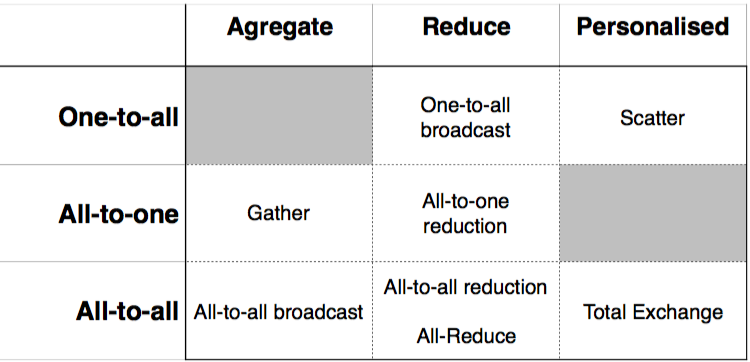
\includegraphics[width=0.5\linewidth]{img/comm_table}
    \caption{Types of global communications}
    \label{fig:commtable}
\end{figure}

\subsection{One-to-All and All-to-One}

\begin{figure}[H]
\centering
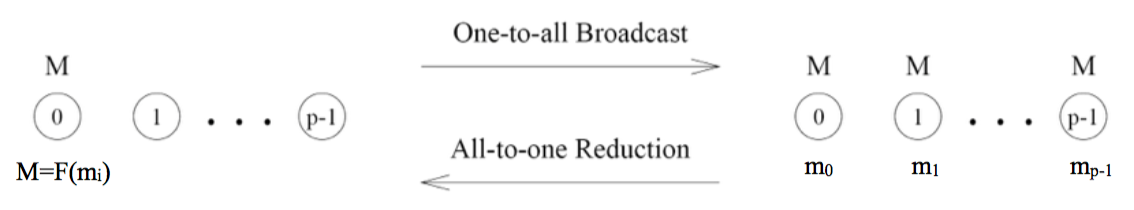
\includegraphics[width=0.7\linewidth]{img/comm_one-to-all}
\caption{One-to-All: ne processor has a piece of data (of size m) it needs to 
send to everyone}
\label{fig:comonetoall}
\end{figure}

All-to-One:

\begin{itemize}
    \item each processor has \(m\) units to broadcast
    \item results made available at target processor
    \item With or without reduction:
    \begin{itemize}
        \item With: data items combined (reduce)
        \item Without: \(m\) increases at each step (glued together, gather)
    \end{itemize}
\end{itemize}

\subsubsection{On Rings}

\begin{itemize}
    \item Naive: send $p-1$ messages from source to other $p-1$ nodes
    \begin{itemize}
        \item source not is bottleneck
        \item network under-utilized
        \item require $p-1$ steps
    \end{itemize}
    
    \item Recursive doubling: at each step the node owning the message sends 
    the message to a selected node
\end{itemize}

\begin{figure}[H]
    \centering
    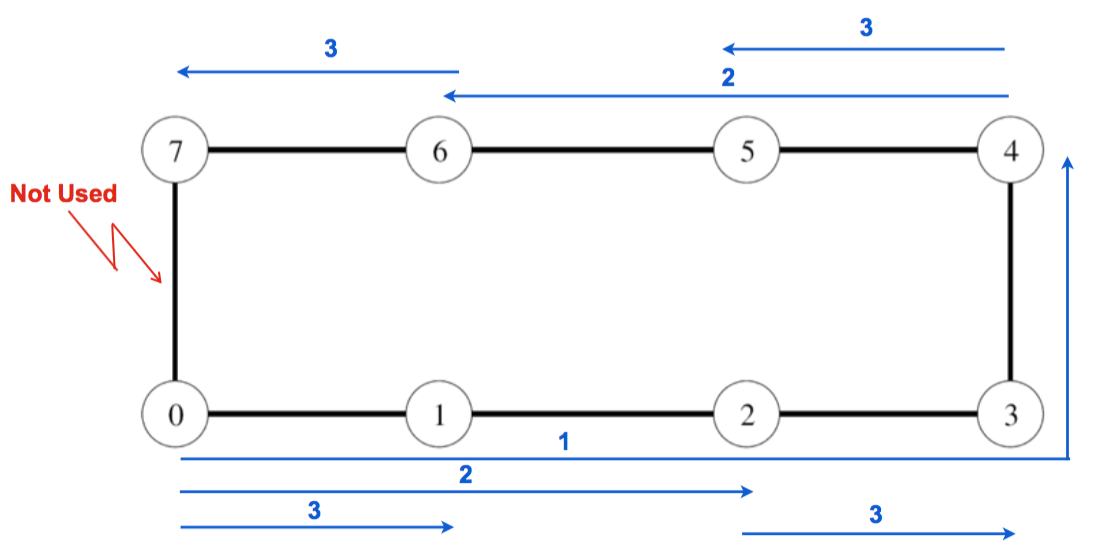
\includegraphics[width=0.7\linewidth]{img/comm_ring_one-to-all}
    \caption{One-to-All on ring. Number on arrow = step where transfer happens}
    \label{fig:commoneallring}
\end{figure}

\begin{figure}[H]
    \centering
    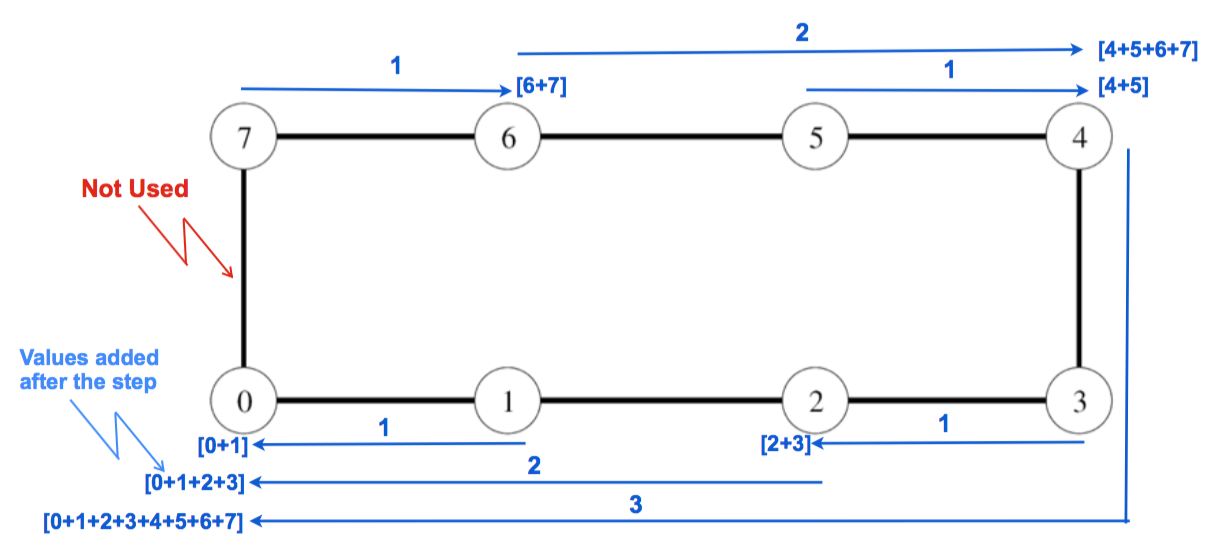
\includegraphics[width=0.7\linewidth]{img/comm_ring_all-to-one}
    \caption{All-to-One on Ring}
    \label{fig:commringall-to-one}
\end{figure}

Number of steps: $ \log{p} = \log{2^N} $

With reduction = Reduce ($m$ constant)

\begin{itemize}
    \item Transmission time for step $i$:
    $ T_{i} = t_{L} + m*t_{W} + H_{i} * t_{S} $
    
    \item Total transmission time:
    $ T = \log{p} * (t_{L} + m*t_{W}) + (p-1) * t_{S}) $
\end{itemize}

Without reduction = Gather ($m$ increases at each step)

\begin{itemize}
    \item Time for step $i$:
    \begin{itemize}
        \item $T_{i} = t_{L} + m_{i} * t_{W} + H_{i} * t_{s}$
        \item $m_{i} = 2^{i} * m$
    \end{itemize}
    \item Total time:
    $T=\log{p}*t_{L} + m(p-1)*t_{W} + (p-1) * t_{S}$
\end{itemize}

\subsubsection{On Mesh, Hypercube}

\begin{figure}[H]
\centering
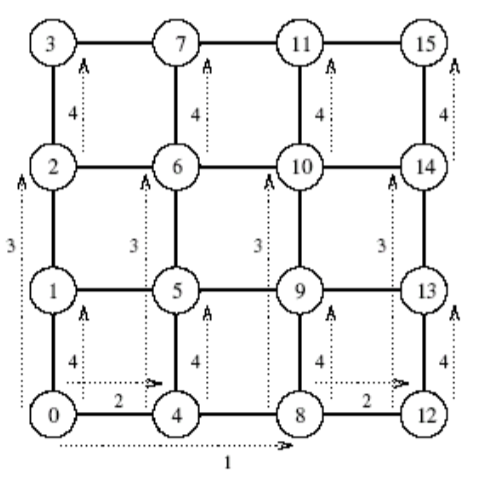
\includegraphics[width=0.5\linewidth]{img/comm_mesh_one-to-all}
\caption{One-to-All on mesh}
\label{fig:commmeshone-to-all}
\end{figure}

Formulas: 
\begin{itemize}
    \item dD-mesh:
    $ \log{p}*(t_{L} + m * t_{W}) + d * (\sqrt[d]{p}-1) * t_{S})$
    
    \item Hypercube ($d=\log{p}$):
    $T = \log{p} * (t_{L} + m * t_{W} + t_{S})$
\end{itemize}


\subsection{All-to-All}

2 types:

\begin{itemize}
    \item All-to-All Broadcast: Each processor $p_{i}$ sends to all others the 
    same $m_{i}$-word message, different processors may broadcast different 
    messages
    \item All-to-All Reduction: every node is the destination of 
an all-to-one reduction, each node starts with p messages
\end{itemize}

\subsubsection{On a ring}

\begin{itemize}
    \item Half of the nodes first sends its message to one of its neighbors to 
    initiate the all-to-all communication.
    
    \item In subsequent steps, each node forwards the [0,4,5,6,7] data he is 
    receiving plus the data he is already owning to its neighbor
    
    \item The algorithm terminates in p steps
\end{itemize}

For reduction, inverted process. On receiving a message, a node must combine  
(for example add) it with its local copy of the value before forwarding the 
value message to the next neighbor.

Costs on ring:

\begin{itemize}
    \item With reduction:
    $T = p*(t_{L} + m*t_{W})$
    
    \item Without reduction:
    $T = p * (t_{L} + t_{W} * m (2p-1))$
\end{itemize}

Read and write at the same time:

\begin{itemize}
    \item All of the nodes first sends its message to one of its neighbors to 
    initiate the all-to-all communication.
    
    \item In subsequent steps, each node forwards the data he is receiving plus 
    the data he is already owning to its neighbor the algorithm terminates in 
    p-1 steps.
    
    \item With or without reduction at each step p messages of size m are sent 
    and received.
\end{itemize}

Total time (with or without reduction): $T = p*(t_{L} + m*t_{W})$

\subsubsection{On a mesh}

\begin{figure}[H]
    \centering
    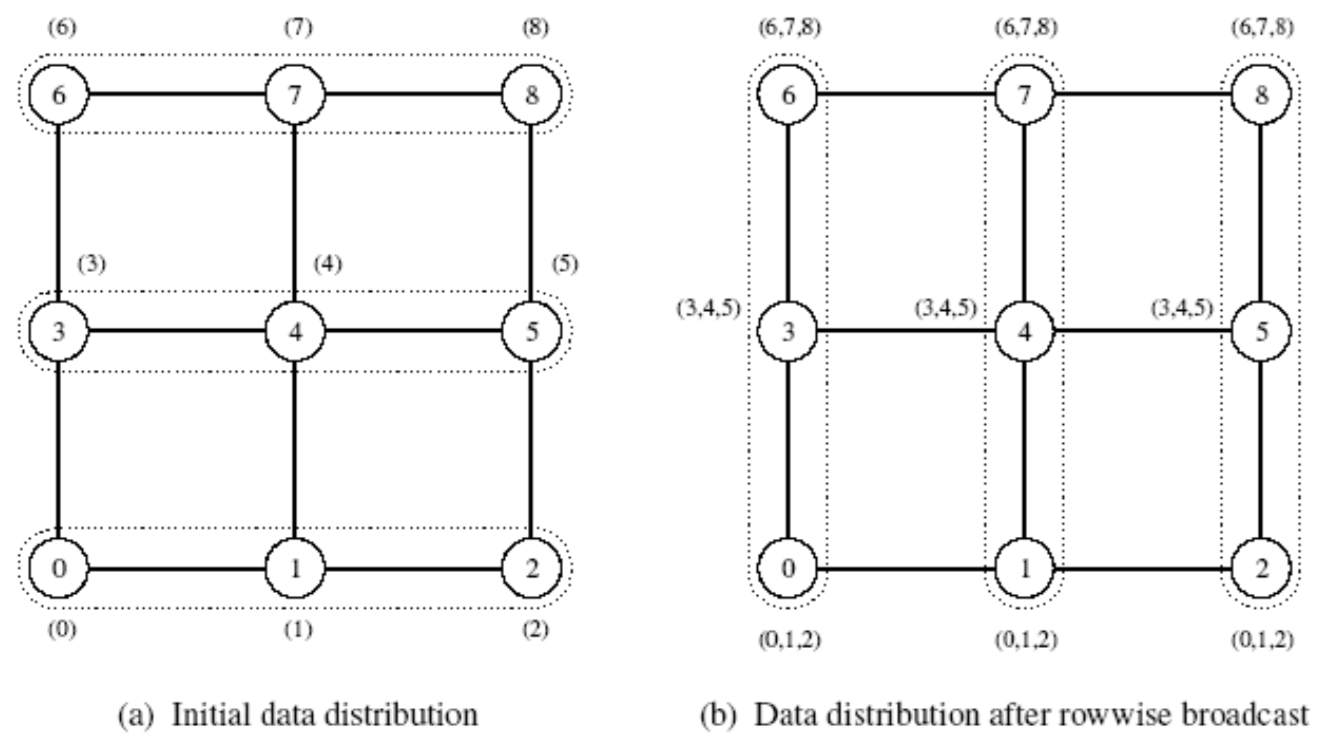
\includegraphics[width=0.7\linewidth]{img/comm_mesh_al-to-all}
    \caption{All-to-All broadcast on a mesh}
    \label{fig:commmeshal-to-all}
\end{figure}

Algorithm:

\begin{enumerate}
    \item Phase 1
    \begin{itemize}
        \item Each row of the mesh performs an all-to-all broadcast using the 
        procedure for the ring
        
        \item In this phase, all nodes collect $\sqrt{p}$ messages 
        corresponding to the $\sqrt{p}$ nodes of their respective rows
    \end{itemize}
    
    \item Phase 2
    \begin{itemize}
        \item Columnwise all-to-all broadcast
    \end{itemize}
\end{enumerate}

Torus is better for routing between the ends of columns/rows.

Cost for Torus:

\begin{itemize}
    \item With reduction: $T = 2(\sqrt{p} * (t_{L} + m *t_{W}))$
    \item Without reduction:
    \begin{itemize}
        \item Phase 1:
        $ \sqrt{p} (t_{L} + t_{W} * m(2\sqrt{p}-1)) $
        
        \item Phase 2:
        $ \sqrt{p} (t_{L} + t_{W} * \sqrt{p} * m(2\sqrt{p}-1)) $
        
        \item Total:
        $ \sqrt{p} * (2t_{L} + m * (2p+\sqrt{p}-1) * t_{W}) $
    \end{itemize}
\end{itemize}

Cost for Torus with R/W in the same step:

\begin{itemize}
    \item Without reduction:
    \begin{itemize}
        \item First phase:
        $ (\sqrt{p}-1) * (t_{L} + m * t_{W}) $
        
        \item Second phase:
        $ (\sqrt{p}-1) * (t_{L} + \sqrt{p} * m * t_{W}) $
        
        \item Total:
        $ T = (\sqrt{p}-1) 2t_{L} + m * t_{W}(p-1) $
    \end{itemize}
    
    \item With reduction: $ T = 2(\sqrt{p}-1) * (t_{L} + m * t_{W}) $
\end{itemize}


\subsection{Total Exchange}

\begin{figure}[H]
\centering
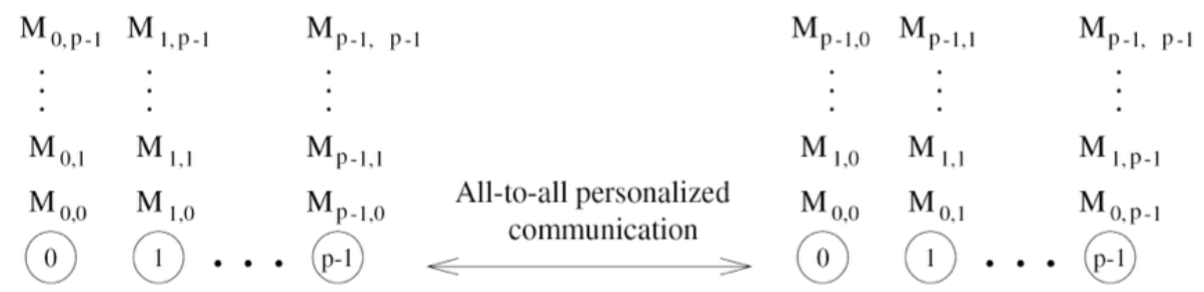
\includegraphics[width=0.7\linewidth]{img/comm_total-exchange}
\caption{Total exchange}
\label{fig:commtotal-exchange}
\end{figure}

\subsubsection{On a ring}

\begin{figure}[H]
    \centering
    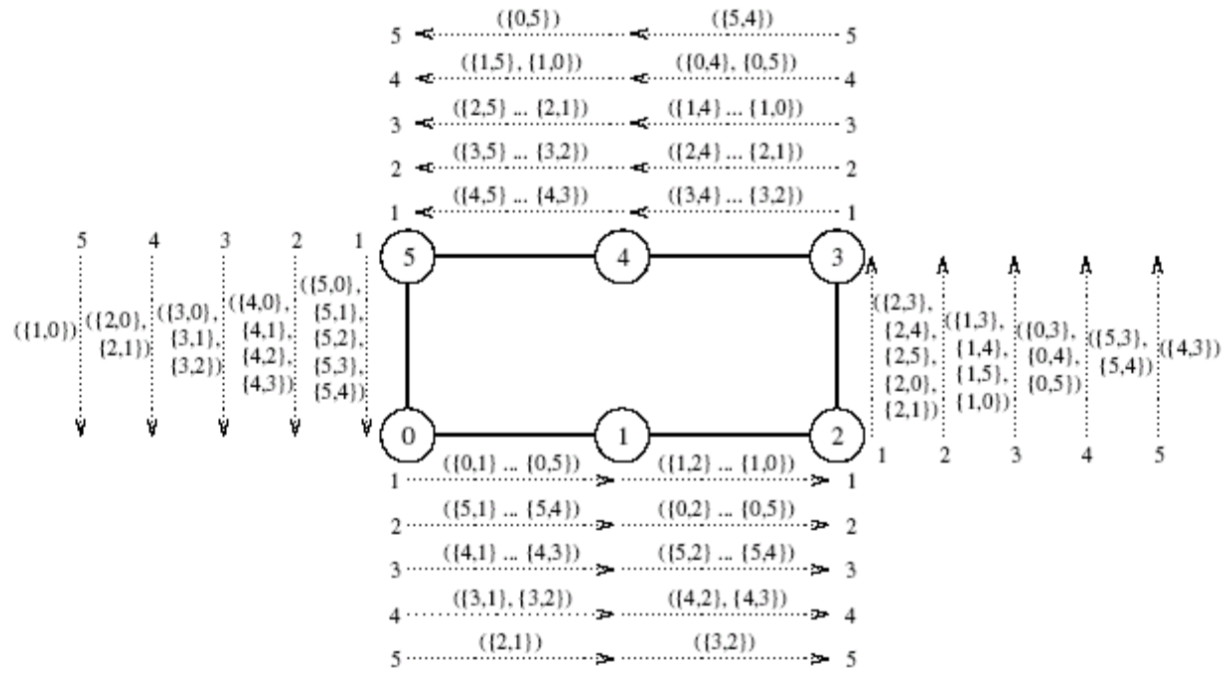
\includegraphics[width=0.7\linewidth]{img/comm_ring_totalexchange}
    \caption{Total exchange ring}
    \label{fig:commringtotalexchange}
\end{figure}

Algorithm:

\begin{enumerate}
    \item Each node sends all pieces of data as one consolidated message of 
    size $m(p - 1)$ to one of its neighbors
    
    \item Each node extracts the information meant for it from the data 
    received, and forwards the remaining pieces of size $m$ each to the next 
    node
    
    \item The size of the consolidated message reduces by $m$ at each step
\end{enumerate}

Cost: $ T = (p-1) * (t_{L} + t_{W} * m * p) $

\subsubsection{On a mesh}

\begin{figure}[H]
    \centering
    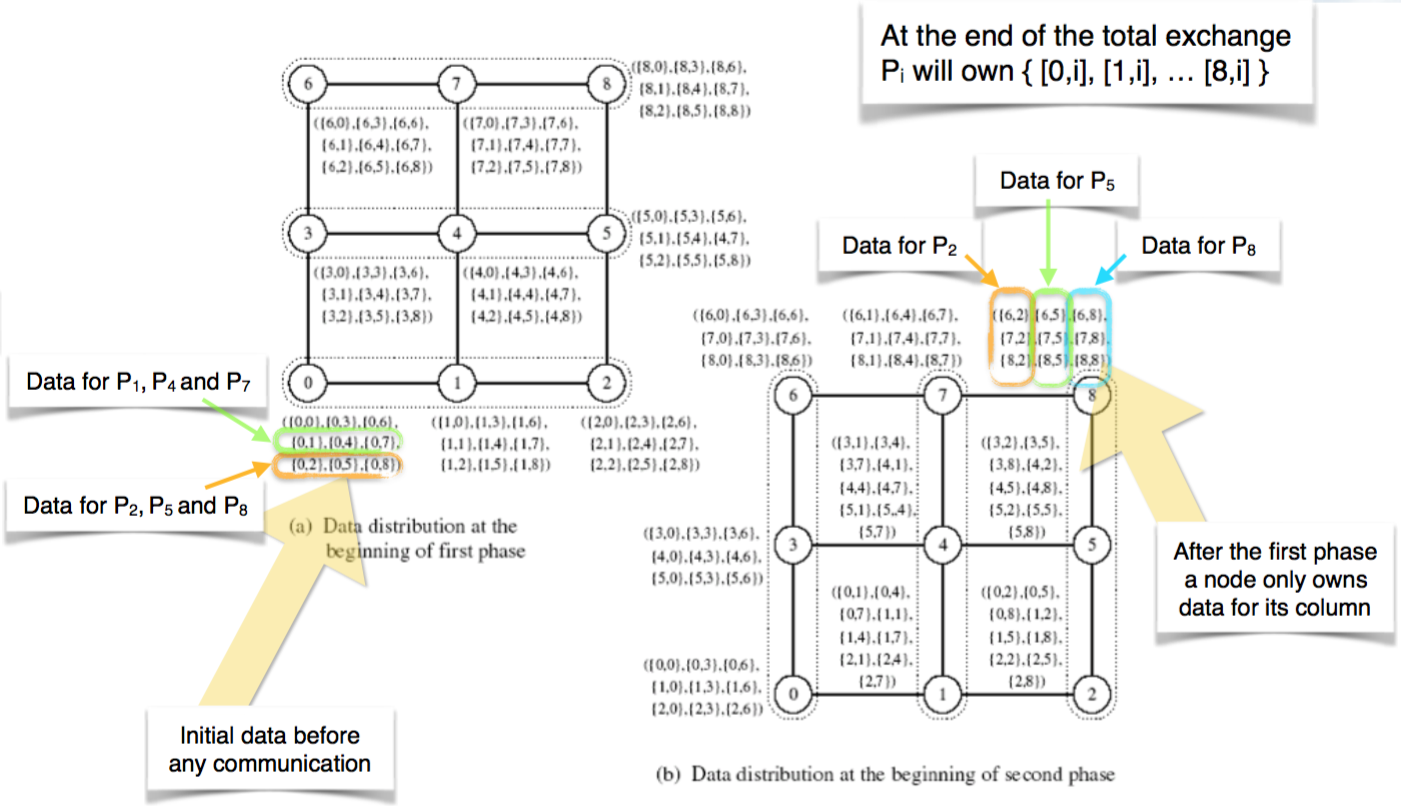
\includegraphics[width=0.7\linewidth]{img/comm_mesh_totalexchange}
    \caption{Total exchange on a Mesh}
    \label{fig:commmeshtotalexchange}
\end{figure}

Algorithm:

\begin{enumerate}
    \item First step
    \begin{itemize}
        \item All-to-All personalized communication is performed independently 
        in each row
        \item Each node of the row keeps all messages for which the destination 
        is inside the column it belongs , it forwards the other ones
    \end{itemize}

    \item Second step
    \begin{itemize}
        \item All-to-All personalized communication is performed independently 
        in each column
        
        \item Each node keeps the messages for which it is the destination, it 
        forwards the other ones
    \end{itemize}
\end{enumerate}

Cost: $ T=(2t_{S} +t_{W}mp)(\sqrt{p} - 1) $

% chapter Communication (end)

\chapter{Sorting algorithms} % (fold)
\label{cha:Sorting algorithms}

\section{Constant time sorting algorithm} % (fold)
\label{sec:Constant time sorting algorithm}

The constant time sorting algorithm is not efficient because is work complexity $ = O(N^2) = O(N \log^{k+1}(N))$. This algorithm is not optimal either. Is surface complexity is $O(H_{//}(A_N)) = O(N^2)$.

% section Constant time sorting algorithm (end)

\section{Sorting network} % (fold)
\label{sec:Sorting network}

A Sorting network is a network of comparators designed specifically for sorting. A comparator is a device with $2$ inputs and $2$ outputs $x_{out} = min(x_{in},y_{in})$ and $y_{out} = max(x_{in},y_{in})$ or the inverse (increasing comparator for first and decreasing comparator for the second).

Every sorting network is made up of a series of columns and each column contains a number of comparators connected in parallel.

\begin{center}
\begin{tikzpicture}
    \node[rectangle,draw] (A) at (0,0) {Input data};
    \node[rectangle,draw,minimum size=1cm] (D) at (2,-2) {};
    \node[rectangle,draw,minimum size=1cm] (B) at (2,0) {};
    \node[rectangle,draw,minimum size=1cm] (C) at (2,2) {};

    \node[rectangle,draw,minimum size=1cm] (D1) at (6,-2) {};
    \node[rectangle,draw,minimum size=1cm] (B1) at (6,0) {};
    \node[rectangle,draw,minimum size=1cm] (C1) at (6,2) {};

    \node[rectangle,draw,minimum size=1cm] (D2) at (8,-2) {};
    \node[rectangle,draw,minimum size=1cm] (B2) at (8,0) {};
    \node[rectangle,draw,minimum size=1cm] (C2) at (8,2) {};

    \node[] (F) at (6,-4) {Column of comparators};


    \node[rectangle,draw] (A1) at (10,0) {Output data};

    \draw (A) -- (B) -- (B1) -- (B2) -- (A1);
    \draw (A) -- (C) -- (C1) -- (C2) -- (A1);
    \draw (A) -- (D) -- (D1) -- (D2) -- (A1);
    \draw[->] (F) -- (D1);
    \draw[->] (F) -- (D);
    \draw[->] (F) -- (D2);


    \node[rectangle,draw,minimum width=6cm,minimum height=1cm, rotate=90] (E) at (3.5,0) {Intercommunication network};
\end{tikzpicture}
\end{center}

A network with $n$ inputs performing a $max$ operation is denoted by $\ominus BM[n]$

\section{Bitonic sort} % (fold)
\label{sec:Bitonic sort}

First, we define what is a bitonic sequence. A bitonic sequence has two tones : increasing then decreasing, or vice versa and any cyclic rotation of a bitonic sequence is also bitonic.

$\langle 1,2,3,7,6,0 \rangle$ and $\langle 9,2,1,0,4,8 \rangle$ are bitonic sequence.

The bitonic sort is the following :
\begin{itemize}
    \item Build a single bitonic sequence from the given unsorted sequence
    \item Rearrange the bitonic sequence into a sorted one
\end{itemize}

A bitonic sorting network sorts $n$ elements in $O(\log^2n)$ time.

To sort a bitonic sequence :
\begin{itemize}
    \item Let $s = \langle a_0,a_1,...,a_{n-1} \rangle$ a bitonic sequence.
    \item Consider the two subset of $s = \{s_1,s_2\}$
        \begin{itemize}
            \item $s_1 = \langle min(a_0,a_{n/2}),min(a_1,a_{n/2 + 1}),... \rangle$.
            \item $s_2 = \langle max(a_0,a_{n/2}),max(a_1,a_{n/2 + 1}),... \rangle$.
        \end{itemize}
    \item $s_1,s_2$ are bitonic sequence too and each element of $s_1$ is less or equals to each element of $s_2$.
    \item Apply the procedure recursively too fully sort $s$.
\end{itemize}

The sorting network which use the bitonic algorithm contains $\log n$ columns and each columns contains $\frac{n}{2}$ comparators. In this case we perform a $min$ operation.

Now we need to transform any sequence into a bitonic ones :
\begin{itemize}
    \item A sequence of length $2$ is always bitonic.
    \item A bitonic sequence of length $4$ by sorting the first two elements using $\oplus BM[2]$ and next two element using $\ominus BM[2]$.
    \item This process can be reapeted to generate larger bitonic sequences.
\end{itemize}

The network of this algorithm contains $\frac{n}{2}$ with a $\oplus BM[2]$ on even place of the horizontal. This algorithm could also be mapped to meshes by performing compare-exchange operation between two wire only ig their labels differ in exactly one bit. The complexity for the mesh is $T_P = O(\log^2n) + O(\sqrt{n})$,this is not the optimal cost.

When each processor hsa more than one value, the compare-exchange operation is replaced by the compare-split operation :

\begin{itemize}
    \item assume each processor have $\frac{n}{p}$ elements.
    \item after the operation, the smaller $\frac{n}{p}$ are at processor $P_i$ and the larger at $P_j$, where $i < j$.
    \item the complexity of a compare-split is $O(\frac{n}{p})$.
    \item the communication time is $t_s + t_w \frac{n}{p}$ (assuming they are neighbour).
    \item when $n$ increase, $t_s$ becomes insignificant.
    \item the global complexity is $O(\frac{n}{p})$.
\end{itemize}

\begin{enumerate}
    \item each process sens its block of size $\frac{n}{p}$ to the other process
    \item each process merges the received block with its own block
    \item each process retains only the appropriate half of the merged block (process $P_i$ retains the smaller elements and $P_j$ the larger)
\end{enumerate}

\paragraph*{Quicksort :} $O(n \log n)$.

\paragraph*{Mergesort :} $O(n \log n)$, but on a PRAM $O(n)$ with $O(T_{//}(A_N)) = O(N^2)$, neither efficient or optimal : communication overhead.

% section Sorting network (end)

% chapter Sorting algorithms (end)

\end{document}
